\section{Auswertung}
\label{sec:Auswertung}

\subsection{Viskosität von Wasser}

Zunächst wird die Dichte der beiden Kugeln berechnet. Für die Kugeln 
ergaben sich die in Tabelle \ref{tab:Dichte} dargestellten Messwerte für den 
Durchmesser und die Masse, sowie die daraus berechneten Werte für das 
jeweilige Volumen und die Dichte.

\begin{table}
\centering
\caption{Messwerte für Durchmesser, Masse und berechnetes Volumen und Dichte}
\label{tab:Dichte}
\sisetup{table-format=2.1}
\begin{tabular}{c c c c}
\toprule
$d \,/\, \si{\milli\meter}$ & $m \,/\, \si{\gram}$ & $V \,/\, \si{\cm³}$ & $\rho \,/\, \si{\frac{g}{cm³}}$\\
\midrule
15.8 &  5.38 & 2.07 & 2.60\\
15.6 &  4.95 & 1.99 & 2.49\\
\bottomrule
\end{tabular}
\end{table}

Zunächst wurde die Fallzeit der kleinen und großen Kugel bei 21.5°C 
jeweils 10 Mal gemessen. 
Die ermittelten Werte sind in Tabelle \ref{tab:Zeit} aufgetragen. 

\begin{table}
\centering
\caption{Messwerte für die Fallzeiten}
\label{tab:Zeit}
\sisetup{table-format=2.1}
\begin{tabular}{c c}
\toprule
$t\: (kleine\: Kugel)\,/\, \si{\second}$ & $t\: (grosse\: Kugel) \,/\, \si{\second}$\\
\midrule
12.47 & 79.95\\
12.53 & 80.32\\
12.33 & 80.27\\
12.29 & 80.10\\
12.12 & 80.04\\
12.38 & 79.84\\
12.46 & 80.15\\
12.53 & 79.18\\
12.46 & 80.15\\
12.41 & 79.92\\
\bottomrule
\end{tabular}
\end{table}

Aus diesen Werten werden Mittelwert und Standardabweichung gebildet.
$t_g$ ist dabei die Fallzeit der großen und $t_k$ die Fallzeit der kleinen
Kugel.

\begin{align*}
t_k &= \SI{12.40+-0.12}{\second}\\
t_g &= \SI{80.00+-0.31}{\second}
\end{align*}

Nun berechnet sich die Viskosität $\eta$ des Wassers nach (\ref{eqn:Viskosität}).
Die Apperaturkonstante der kleinen Kugel ist gegeben mit 

\begin{equation*}
K_k = \SI{0.0764}{\milli\pascal\cubic\centi\meter\per\gram}
\end{equation*}

Mit der Gaußschen Fehlerfortpflanzung

\begin{align}
\Delta \eta &= \sqrt{\left(\frac{\partial\eta}{\partial t}\right)^2 \cdot \left(\Delta t\right)²}\\
&=\sqrt{\left(K\cdot(\rho_K - \rho_F)\right)²\cdot(\Delta t)²}
\end{align}

und der Dichte des Wassers 

\begin{equation}
\rho _F = \SI{998.8}{\kilo\gram\per\cubic\meter}
\end{equation}

ergibt sich folgender Wert für die Viskosität $\eta$:

\begin{equation*}
\eta = \SI{0.001413+-0.000014}{\kilo\gram\per(\meter\second)}
\end{equation*}

Aus diesem Wert kann die Apperaturkonstante $K$ der großen Kugel
bestimmt werden. Dafür wird die Formel \ref{eqn:Viskosität} nach 
$K$ umgestellt: 

\begin{equation*}
K = \frac{\eta}{(\rho_K - \rho_F) \cdot t}
\end{equation*}

Mit der Gaußschen Fehlerfortpflanzung

\begin{align*}
\Delta K &= \sqrt{\left(\frac{\partial K}{\partial \eta}\cdot \Delta\eta\right)² + \left(\frac{\partial K}{\partial t}\cdot \Delta t\right)²}\\
&= \sqrt{\left(\frac{1}{(\rho_K - \rho_F)\cdot t}\cdot \Delta\eta\right)² + \left(\frac{-\eta}{(\rho_K - \rho_F)\cdot t²}\cdot \Delta t\right)²}
\end{align*}

ergibt sich für K: 

\begin{equation*}
K = \SI{493.40+-5e-9}{\meter\squared\per\second\squared}
\end{equation*}

\subsection{Temperaturabhängigkeit der Viskosität}

Die für 10 Temperaturen zwischen 21°C und 70°C gemessenen Fallzeiten 
sind in Tabelle \ref{tab:Temperatur} eingetragen.

\begin{table}
\centering
\caption{Temperaturabhängige Fallzeiten und Viskositäten}
\label{tab:Temperatur}
\sisetup{table-format=2.1}
\begin{tabular}{c c c c c c}
\toprule
$T \,/\, \si{\kelvin}$ & $\frac{1}{T} \,/\, \si{\milli\kelvin^{-1}}$& \multicolumn{2}{c}{t \,/\, \si{\second}} & $\overline{t}$ & $\eta \,/\, \si{\gram\per\second\meter}$\\
\midrule
300.15 & 3.33 & 72.00 & 71.18 & 71.59 \pm\:0.41 & 52.70 \pm\:0.60\\
304.15 & 3.29 & 66.13 & 65.47 & 65.80 \pm\:0.33 & 48,40 \pm\:0.50\\
308.15 & 3.25 & 61.93 & 60.90 & 61.42 \pm\:0.52 & 45.20 \pm\:0.60\\
315.15 & 3.17 & 53.89 & 53.58 & 53.74 \pm\:0.16 & 39.50 \pm\:0.40\\
319.65 & 3.13 & 49.50 & 49.77 & 49.64 \pm\:0.14 & 36.50 \pm\:0.40\\
323.65 & 3.09 & 44.95 & 46.20 & 45.58 \pm\:0.63 & 33.50 \pm\:0.60\\
328.15 & 3.05 & 43.30 & 43.16 & 43.23 \pm\:0.07 & 31.81 \pm\:0.33\\
333.15 & 3.00 & 40.30 & 40.29 & 40.30 \pm\:0.01 & 29.65 \pm\:0.30\\
338.15 & 2.96 & 38.43 & 37.80 & 38.11 \pm\:0.32 & 28.00 \pm\:0.40\\
343.15 & 2.91 & 36.40 & 36.18 & 36.29 \pm\:0.11 & 26.63 \pm\:0.28\\
\bottomrule
\end{tabular}
\end{table}

In der Tabelle sind die jeweiligen Mittelwerte der Fallzeiten mit deren Standardabweichung
aus den beiden Messungen für eine Temperatur aufgeführt. Außerdem wird die 
jeweilige Viskosität nach Formel (\ref{eqn:Viskosität}) ausgerechnet und deren
Fehler durch die Gaußsche Fehlerfortpflanzung nach (6) und (7) berechnet. 

Nun wird $ln(\eta)$ gegen $1/T$ in Abbildung \ref{fig:plot} aufgetragen.

\begin{figure}
  \centering
  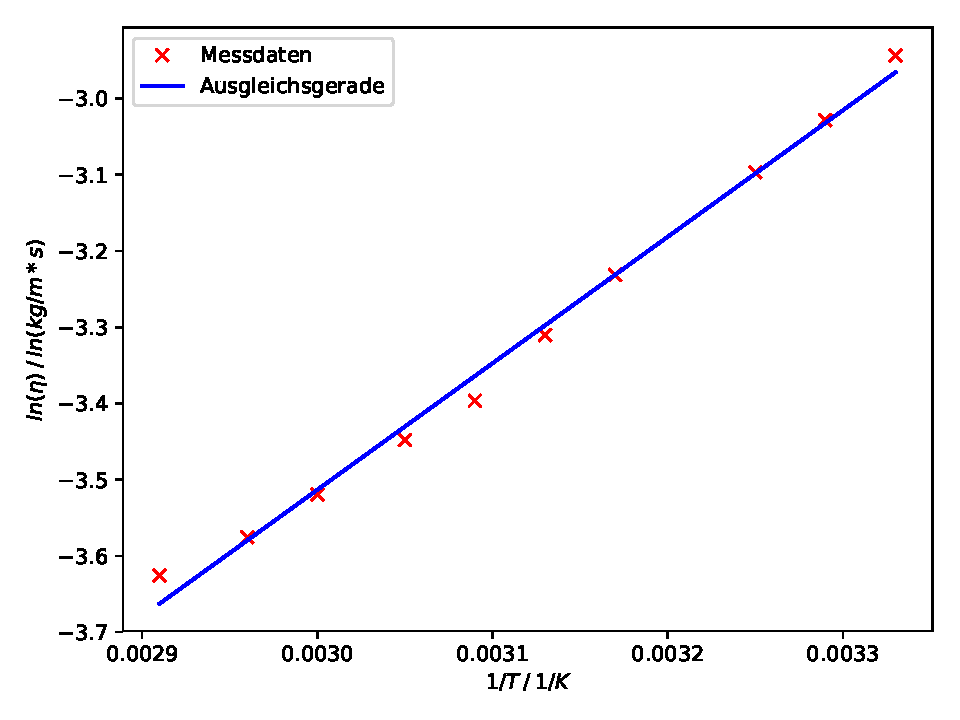
\includegraphics[scale=0.7]{content/plot1.pdf}
  \caption{Temperaturabhängigkeit der Viskosität}
  \label{fig:plot}
\end{figure}

Die lineare Regression, durchgeführt mit Python und Numpy, 
liefert folgende Geradengleichung: 

\begin{equation*}
\ln{(\eta)} = B\cdot \frac{1}{T} + \ln{(A)}
\end{equation*}

Dabei ergeben sich die Parameter A und B aus der Andradeschen Gleichung zu: 

\begin{align*}
A &= \exp{(-8.492\pm0.1756)} = (\num{2.05e-4}\pm\num{3.60e-5})\si{\kilo\gram\per\meter\per\second} \\
B &= \SI{1659.546+-56.2745}{\kelvin}
\end{align*}

Für die Zeitabhängigkeit der Viskosität gilt also:

\begin{equation*}
\eta (T) = (\num{2.05e-4})\si{\kilo\gram\per\meter\per\second} \cdot \exp{\left(\frac{\SI{1659.546}{\kelvin}}{T}\right)}
\end{equation*}

\subsection{Reynolds Zahl}

Mit den berechneten Werten lässt sich nun die Reynoldszahl für die 
jeweiligen Temperaturen berechnen. Die Ergebnisse für die große Kugel sind 
in Tabelle \ref{tab:Zeit} aufgeführt.

\begin{table}
\centering
\caption{Temperaturabhängige Reynoldszahl}
\label{tab:Zeit}
%\sisetup{table-format=2.1}
\begin{tabular}{S[table-format=3.2] S[table-format=1.3]@{${}\pm{}$}S[table-format=1.3] 
S[table-format=2.2]@{${}\pm{}$}S[table-format=1.2]}
\toprule
{$T\,/\, \si{\kelvin}$} & \multicolumn{2}{c}{$v\,/\, \si{\milli\meter\per\second}$} 
& \multicolumn{2}{c}{$Re$}\\
\midrule
300.15 & 1.397 & 0.008 &  4.18 & 0.05\\
304.15 & 1.520 & 0.008 &  4.96 & 0.06\\
308.15 & 1.682 & 0.014 &  5.68 & 0.09\\
315.15 & 1.861 & 0.006 &  7.44 & 0.08\\
319.65 & 2.015 & 0.006 &  8.71 & 0.10\\
323.65 & 2.199 & 0.030 & 10.36 & 0.23\\
328.15 & 2.313 & 0.004 & 11.47 & 0.12\\
333.15 & 2.481 & 0.001 & 13.20 & 0.13\\
338.15 & 2.624 & 0.022 & 14.79 & 0.24\\
343.15 & 2.762 & 0.008 & 16.37 & 0.18\\
\bottomrule
\end{tabular}
\end{table}

Außerdem ergibt sich die Reynoldzahl für die kleine Kugel: 

\begin{equation*}
Re_{kl} = \num{890.7+-1.1}
\end{equation*}

Es ist zu erkennen, dass die Reynoldzahl für alle Temperaturen unter 1160 
liegt und man somit von laminaren Stömungsverhältnissen ausgehen kann.